\documentclass[11pt,letterpaper]{article}
\usepackage[lmargin=1in,rmargin=1in,tmargin=1in,bmargin=1in]{geometry}
\usepackage{../style/homework}
\usepackage{../style/commands}
\setbool{quotetype}{false} % True: Side; False: Under
\setbool{hideans}{false} % Student: True; Instructor: False

% -------------------
% Content
% -------------------
\begin{document}

\homework{11: Due 04/14}{The power of mathematics is often to change one thing into another, to change geometry into language.}{Marcus du Sautoy}

% Problem 1
\problem{10} The speed of an airplane is 821.3~ft/s. Find this speed in miles per hour (mph). [Note: 5280~ft $=$ 1~mi] \pspace

\sol 
	\begin{table}[!ht]
	\centering
	\begin{tabular}{r|r|r|r}
	821.3~ft & 1~mi & 60~s & 60~min \\ \hline
	1~s	     & 5280~ft & 1~min & 1~hr
	\end{tabular}
	= 559.977~mph
	\end{table}



\newpage



% Problem 2
\problem{10} Find $x$ in the diagram below:
	\[
	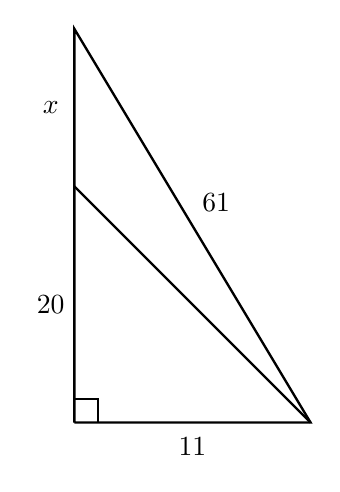
\begin{tikzpicture}
	\draw[line width=0.03cm] (0,0) -- (0,5) -- (3,0) -- (0,0);
	\draw[line width=0.03cm] (0,0.3) -- (0.3,0.3) -- (0.3,0);
	\draw[line width=0.03cm] (3,0) -- (0,3);
	\node at (1.5,-0.3) {$11$};
	\node at (-0.3,1.5) {$20$};
	\node at (1.8,2.8) {$61$};
	\node at (-0.3,4.0) {$x$};
	\end{tikzpicture}
	\]

\sol The large triangle is a right triangle. Therefore, by the Pythagorean Theorem, $a^2 + b^2= c^2$, where $a$ and $b$ are the legs of the triangle and $c$ is the hypotenuse. The larger triangle has legs $11$ and $x + 20$ and hypotenuse $61$. But then we have\dots
	\[
	\begin{aligned}
	(x + 20)^2 + 11^2&= 61^2 \\[0.3cm]
	(x + 20)^2 + 121&= 3721 \\[0.3cm]
	(x + 20)^2&= 3600 \\[0.3cm]
	\sqrt{(x + 20)^2}&= \sqrt{3600} \\[0.3cm]
	x + 20&= 60 \\[0.3cm]
	x&= 40
	\end{aligned}
	\]



\newpage



% Problem 3
\problem{10} A `track' consists of two semicircles adjoined to the sides of a rectangle. Find the perimeter and the area of the `track' below.
	\[
	\begin{tikzpicture}
	\draw[line width=0.03cm] (0,0) -- (8,0);
	\draw[line width=0.03cm] (0,4) -- (8,4);
	\draw[line width=0.03cm] (8,4) -- (8,0) arc(-90:90:2);
	\draw[line width=0.03cm] (0,0) -- (0,4) arc(90:270:2);
	\draw[line width=0.04cm,white] (0,0.015) -- (0,3.985);
	\draw[line width=0.03cm,dotted] (0,0.015) -- (0,3.985);
	\draw[line width=0.04cm,white] (8,0.015) -- (8,3.985);
	\draw[line width=0.03cm,dotted] (8,0.015) -- (8,3.985);
	\node at (4,-0.3) {$88$~m};
	\node at (0.6,2) {$46$~m};
	\end{tikzpicture}
	\] \pspace

\sol The region above consists of two half circles and a rectangle. The perimeter is the distance around the figure. The two circle halves can be combined into one circle with diameter 46~m, i.e. radius 23~m. The perimeter of a circle is $2\pi r$. Only the upper and lower sides of the rectangle are included in the perimeter. Therefore, the perimeter is\dots
	\[
	P= 2\pi r + 2h= 2 \pi \cdot 23 + 2 \cdot 88= 46\pi + 176 \approx 320.513 \text{ m}
	\]
The area of the above figure can be broken into the area from the rectangle and the area from two half circles, i.e. one whole circle. The area of a rectangle is $bh$ and the area of a circle is $\pi r^2$. Therefore, we have\dots
	\[
	A= \pi r^2 + bh= \pi \cdot 23^2 + 88(46)= 529\pi + 4048 \approx 5709.9 \text{ m}^2
	\]


\end{document}